\documentclass[11pt,a4paper]{article}

\usepackage[utf8]{inputenc}
\usepackage[margin=2.5cm]{geometry}
\usepackage{amsmath,amssymb}
\usepackage{graphicx}
\usepackage{booktabs}
\usepackage{enumitem}
\usepackage{hyperref}
\usepackage{natbib}
\usepackage{tikz}
\usetikzlibrary{arrows.meta,positioning,fit,backgrounds,calc}
\usepackage{xcolor}

% Colors for diagram
\definecolor{memblue}{HTML}{DBEAFE}
\definecolor{trustorange}{HTML}{FED7AA}
\definecolor{beliefgreen}{HTML}{D1FAE5}
\definecolor{envpink}{HTML}{FCE7F3}
\definecolor{commpurple}{HTML}{EDE9FE}
\definecolor{normyellow}{HTML}{FEF3C7}
\definecolor{lockinpink}{HTML}{F5D0FE}

\title{\textbf{Cognitive Lock-in and Social Amplification:\\A Unified Model of Norm Emergence}}
\author{}
\date{}

\begin{document}
\maketitle

\begin{abstract}
We present a model of norm emergence in coordination games that combines two mechanisms: \emph{cognitive lock-in} through trust-modulated adaptive memory, and \emph{social amplification} through communication. Individually, cognitive lock-in explains why norms are \emph{stable} once formed---trust expands memory windows, stabilizing beliefs against reversal. Communication explains why norms emerge \emph{quickly}---observations and normative signals accelerate the transition from random behavior to consensus. Neither mechanism alone produces a full social norm in the sense of \citet{bicchieri2006grammar}: cognitive lock-in without communication yields slow-forming conventions lacking normative expectations; communication without lock-in yields fragile consensus vulnerable to perturbation. Together, they produce self-reinforcing norms with both behavioral regularity and shared normative expectations.
\end{abstract}

% =====================================================================
\section{Introduction}
% =====================================================================

Starting from a \textbf{cold start}---50-50 random strategy distribution, no shared history---how does randomness become a social norm? Not merely behavioral convergence, but a self-enforcing pattern sustained by mutual expectations.

Two findings from behavioral and neural science frame our approach. First, \citet{behrens2007learning} showed that the anterior cingulate cortex tracks environmental volatility and adjusts learning rate accordingly. In volatile environments, humans shorten their effective ``memory window,'' prioritizing recent experience over distant history. Second, the social learning strategies tournament \citep{rendell2010copy} showed that the winning strategy is \emph{copy when uncertain}: use social information when individual learning is unreliable, and rely on personal experience when confident.

We unify these insights into a model with two layers:

\begin{enumerate}[itemsep=2pt]
    \item \textbf{Cognitive lock-in} (individual level): Trust, updated by prediction accuracy, controls memory window size. Successful coordination $\to$ higher trust $\to$ longer memory $\to$ more stable beliefs $\to$ resistance to reversal. Action selection uses probability matching---trust affects only \emph{cognition}, not behavior directly.

    \item \textbf{Social amplification} (population level): Communication channels---observations of others' behavior, normative signals expressing what one \emph{should} do, and pre-play signals of intended action---modulate trust dynamics and provide additional information for belief formation. Trust determines the weight given to social vs.\ personal information.
\end{enumerate}

The central claim: \emph{cognitive lock-in explains norm stability; social amplification explains norm speed. Together, they produce true social norms---not just conventions.}

% =====================================================================
\section{Base Model: Cognitive Lock-in}
% =====================================================================

\subsection{Environment}

\begin{itemize}[itemsep=2pt]
    \item $N$ agents (even), strategy set $S = \{A, B\}$
    \item Pure coordination game: payoff 1 if both choose same strategy, 0 otherwise
    \item Each time step $t$: agents randomly paired, simultaneous strategy choice
    \item Agents are anonymous: only partner's strategy is observed, not identity
\end{itemize}

\subsection{Agent State}

Each agent $i$ at time $t$ maintains two state variables:

\begin{table}[h]
\centering
\begin{tabular}{lll}
\toprule
\textbf{State} & \textbf{Symbol} & \textbf{Definition} \\
\midrule
Memory & $M_i(t)$ & Ordered list of recent interactions \\
Trust & $T_i(t) \in [0, 1]$ & Confidence in environment predictability \\
\midrule
\multicolumn{3}{l}{\textit{Derived quantities:}} \\
Belief & $\mathbf{b}_i(t) = [b_A, b_B]$ & Computed from $M_i(t)$ and social information \\
Window & $w_i(t) \in [\text{base}, \text{max}]$ & Computed from $T_i(t)$ \\
\bottomrule
\end{tabular}
\end{table}

Note: unlike the dual-feedback model where temperature $\tau$ is the state variable and trust is derived, here \textbf{trust is the direct state variable}. This eliminates the confound between behavioral effects ($\tau$ controlling softmax randomness) and cognitive effects ($\tau$ controlling memory), enabling clean attribution.

\subsection{One Interaction Cycle}

\paragraph{Step 1: Belief Formation.}
Compute belief from memory by counting observed partner strategies within the effective window:
\begin{equation}
b_A = \frac{n_A}{|M'_i(t)|}, \quad b_B = 1 - b_A
\end{equation}
where $n_A$ is the count of strategy $A$ in effective memory $M'_i(t)$. When memory is empty, belief defaults to $[0.5, 0.5]$.

\paragraph{Step 2: Prediction.}
Agent predicts partner's strategy:
\begin{equation}
\hat{s}_i = \arg\max_{s \in \{A,B\}} b_s
\end{equation}

\paragraph{Step 3: Action Selection (Probability Matching).}
Agent samples from belief distribution:
\begin{equation}\label{eq:prob_matching}
P(s_i = A) = b_A, \quad P(s_i = B) = b_B
\end{equation}
This is \textbf{behaviorally neutral}: if the population is 70\% strategy $A$, the agent plays $A$ with 70\% probability. There is no behavioral amplification at the individual level.

\paragraph{Step 4: Interaction.}
Agent $i$ paired with agent $j$. Both choose simultaneously. Agent $i$ observes partner's strategy $s^*_j$ and coordination outcome.

\paragraph{Step 5: Trust Update.}
Compare prediction $\hat{s}_i$ with observation $s^*_j$:
\begin{equation}\label{eq:trust_update_base}
T_i(t+1) = \begin{cases}
T_i(t) + \alpha \cdot (1 - T_i(t)) & \text{if } \hat{s}_i = s^*_j \quad \text{(correct)} \\[6pt]
T_i(t) \cdot (1 - \beta) & \text{if } \hat{s}_i \neq s^*_j \quad \text{(wrong)}
\end{cases}
\end{equation}

\textbf{Key asymmetry} \citep{slovic1993perceived}: trust builds slowly (additive, saturating) but breaks quickly (multiplicative, proportional to current level). Higher trust means more ``to lose.''

\paragraph{Step 6: Memory Update.}
Append new interaction to memory. If $|M_i| > \text{max\_size}$: remove oldest (FIFO).

\subsection{Trust--Memory Linkage}

For dynamic memory, the effective window depends on trust:
\begin{equation}\label{eq:window}
w_i(t) = \text{base} + \lfloor T_i(t) \times (\text{max} - \text{base}) \rfloor
\end{equation}

The upper bound $\text{max} \approx 6$ reflects working memory limits \citep{miller1956magical}.

\subsection{Trust Steady State}

At equilibrium, $\mathbb{E}[\Delta T] = 0$. Let $p$ denote prediction accuracy ($\approx$ majority fraction):
\begin{equation}\label{eq:trust_steady}
T^* = \frac{p\alpha}{p\alpha + (1-p)\beta}
\end{equation}

With $\alpha = 0.1$, $\beta = 0.3$:

\begin{center}
\begin{tabular}{cccc}
\toprule
Majority $p$ & Trust $T^*$ & Window & Regime \\
\midrule
50\% & 0.25 & 3 & Uncertain, adaptive \\
70\% & 0.44 & 4 & Moderate \\
90\% & 0.75 & 5 & Confident, stable \\
\bottomrule
\end{tabular}
\end{center}

\subsection{The Cognitive Lock-in Mechanism}

Probability matching is behaviorally neutral, yet trust creates \textbf{asymmetric resilience}:
\begin{center}
Majority forms (by drift) $\;\to\;$ Prediction accuracy $\uparrow$ $\;\to\;$ Trust $\uparrow$ $\;\to\;$ Window $\uparrow$ $\;\to\;$ Beliefs stabilize $\;\to\;$ Norm resilience $\uparrow$
\end{center}

Once beliefs stabilize with a large window, random fluctuations are averaged out. The norm becomes resistant to reversal---not because agents amplify the majority behaviorally, but because their \emph{cognitive state} locks in the current equilibrium.

\textbf{Limitation}: Convergence is slow. Without behavioral amplification, norm emergence relies on random drift to break symmetry. This is where communication enters.

% =====================================================================
\section{Communication Extension: Social Amplification}
% =====================================================================

\subsection{Information Sources}

Beyond direct experience, agents can access three communication channels:

\begin{table}[h]
\centering
\small
\begin{tabular}{llll}
\toprule
\textbf{Source} & \textbf{Content} & \textbf{Persistence} & \textbf{Theoretical Basis} \\
\midrule
Direct memory & What happened to me & Window-limited & --- \\
Observations & What I saw others do & Ephemeral (per tick) & \citet{henrich1998conformist} \\
Normative signals & What others think I should do & Expectation array & \citet{bicchieri2006grammar} \\
Pre-play signals & What my partner will do & Single-use & \citet{skyrms2010signals} \\
\bottomrule
\end{tabular}
\end{table}

\subsection{Trust-Modulated Belief Integration}

The key principle: \emph{copy when uncertain} \citep{rendell2010copy}. Trust serves as the reliability index---high trust means individual experience is reliable (use memory); low trust means the environment is volatile (use social information).

Following \citet{toelch2015informational}, we maintain two parallel pathways:

\paragraph{Empirical pathway} (what others do):
\begin{align}
\mathbf{b}^{\text{mem}}_i &= \text{Memory.get\_distribution}() \label{eq:mem_belief} \\
\mathbf{b}^{\text{obs}}_i &= \text{aggregate}(\text{observations}) \label{eq:obs_belief} \\
\omega^{\text{mem}} &= 0.5 + 0.4 \cdot T_i \quad \in [0.5, 0.9] \label{eq:mem_weight} \\
\omega^{\text{obs}} &= 1 - \omega^{\text{mem}} \quad \in [0.1, 0.5] \label{eq:obs_weight} \\
\mathbf{b}^{\text{emp}}_i &= \omega^{\text{mem}} \cdot \mathbf{b}^{\text{mem}}_i + \omega^{\text{obs}} \cdot \mathbf{b}^{\text{obs}}_i \label{eq:emp_belief}
\end{align}

This implements \citeauthor{behrens2007learning}'s (\citeyear{behrens2007learning}) volatility-adjusted learning rate: high trust (low volatility) $\to$ rely on memory; low trust (high volatility) $\to$ rely on social information.

\paragraph{Normative pathway} (what others think I should do):
\begin{align}
\mathbf{b}^{\text{norm}}_i &= \text{normative\_expectation}_i \label{eq:norm_belief} \\
c_i &= \max(\mathbf{b}^{\text{norm}}_i) \quad \text{(consensus strength)} \label{eq:consensus} \\
\omega^{\text{norm}} &= \omega_0^{\text{norm}} \cdot (1 - T_i) \cdot c_i \label{eq:norm_weight}
\end{align}

Normative influence is strongest when trust is low (uncertain agents seek social guidance) \emph{and} consensus is strong (clear normative signal).

\paragraph{Combined belief}:
\begin{equation}\label{eq:combined_belief}
\mathbf{b}_i = (1 - \omega^{\text{norm}}) \cdot \mathbf{b}^{\text{emp}}_i + \omega^{\text{norm}} \cdot \mathbf{b}^{\text{norm}}_i
\end{equation}

\paragraph{Signal override} (immediate coordination):
If a pre-play signal is received with confidence $\phi$:
\begin{align}
\omega^{\text{sig}} &= \phi \cdot (1 - 0.5 \cdot T_i) \label{eq:sig_weight} \\
\mathbf{b}^{\text{final}}_i &= (1 - \omega^{\text{sig}}) \cdot \mathbf{b}_i + \omega^{\text{sig}} \cdot \mathbf{b}^{\text{sig}} \label{eq:final_belief}
\end{align}

The final belief $\mathbf{b}^{\text{final}}_i$ replaces raw memory belief in the action selection rule (Eq.~\ref{eq:prob_matching}).

\subsection{Communication as Trust Feedback Modulator}

Communication does not enter memory. Instead, it \textbf{modulates the trust dynamics} that control memory:

\begin{equation}\label{eq:trust_update_full}
\Delta T_i = \underbrace{\delta^{\text{base}}}_{\text{individual}} \times \underbrace{(1 + \gamma_{\text{obs}} \cdot a_i)}_{\text{social amplification}} - \underbrace{\delta \cdot \mathbf{1}[s_i \neq s^{\text{norm}}] \cdot c_i^2}_{\text{normative pressure}}
\end{equation}

where:
\begin{align}
\delta^{\text{base}} &= \begin{cases}
+\alpha(1 - T_i) & \text{if prediction correct} \\
-\beta \cdot T_i & \text{if prediction wrong}
\end{cases} \label{eq:base_delta} \\
a_i &= 2 \cdot \frac{\#\text{observations matching prediction}}{\#\text{observations}} - 1 \quad \in [-1, 1] \label{eq:alignment}
\end{align}

\begin{itemize}[itemsep=2pt]
    \item $\gamma_{\text{obs}}$: observation amplification factor (default 0.3)
    \item $\delta$: normative pressure strength (default 0.2)
    \item $c_i^2$: nonlinear consensus threshold---weak norms exert little pressure, strong norms are powerful \citep{centola2018tipping}
    \item $s^{\text{norm}}$: majority strategy in normative messages
\end{itemize}

\textbf{Design rationale}: Memory stores only what you experienced directly. Communication modulates \emph{how you learn}, not \emph{what you remember}. This matches \citet{behrens2008social}, who showed that social and reward information produce separate prediction errors in ACC, but both modulate the same learning rate.

% =====================================================================
\section{Three Coupled Feedback Loops}
% =====================================================================

The unified model has three feedback loops, each operating at a different level:

\subsection{Loop 1: Individual Learning (Cognitive Lock-in)}

\begin{center}
Correct prediction $\to$ $T \uparrow$ $\to$ window $\uparrow$ $\to$ beliefs stabilize $\to$ better predictions
\end{center}

This is the V3 base mechanism. It operates through cognition only (no behavioral amplification). Convergence is slow but produces robust, resilient norms.

\textbf{Steady state}: $T^* = p\alpha / (p\alpha + (1-p)\beta)$ (Eq.~\ref{eq:trust_steady}).

\textbf{References}: \citet{slovic1993perceived} for asymmetric trust; \citet{behrens2007learning} for volatility-adjusted learning.

\subsection{Loop 2: Social Amplification (Observations)}

\begin{center}
Agent succeeds $\to$ visible to observers $\to$ others shift beliefs toward agent's strategy $\to$ more partners match agent $\to$ agent succeeds \emph{more} $\to$ trust rises \emph{faster}
\end{center}

Observations amplify \emph{both} positive and negative feedback via the multiplier $(1 + \gamma_{\text{obs}} \cdot a_i)$:
\begin{itemize}[itemsep=0pt]
    \item Aligned with observations: trust dynamics multiplied by up to $(1 + \gamma_{\text{obs}})$
    \item Misaligned: trust dynamics multiplied by down to $(1 - \gamma_{\text{obs}})$
\end{itemize}

This maps to \citeauthor{toyokawa2019conformist}'s (\citeyear{toyokawa2019conformist}) conformist social learning model:
\begin{equation}\label{eq:toyokawa}
P(s) = (1-\sigma) \cdot \text{softmax}(Q_s) + \sigma \cdot \frac{f_s^\theta}{\sum_j f_j^\theta}
\end{equation}
where $\sigma$ (copying weight) maps to $(1 - T_i)$ and $\theta > 1$ (conformity exponent) creates nonlinear majority amplification.

\subsection{Loop 3: Normative Pressure (Signaling)}

\begin{center}
Majority forms $\to$ agents broadcast ``we should do $X$'' $\to$ consensus grows $\to$ minority faces pressure $\to$ switches faster $\to$ majority strengthens $\to$ \textbf{lock-in}
\end{center}

This loop creates additional positive feedback with \textbf{threshold dynamics}. The $c^2$ term in Eq.~\ref{eq:trust_update_full} means:
\begin{itemize}[itemsep=0pt]
    \item Below consensus threshold: little effect (weak norms don't propagate)
    \item Above threshold: powerful cascade (strong norms are self-enforcing)
\end{itemize}

\citet{centola2018tipping} showed experimentally that $\sim$25\% committed minority suffices to tip social conventions. The nonlinear threshold captures this dynamics.

\textbf{Critical distinction}: Without Loop 3, the model produces \emph{conventions} (behavioral regularity). With Loop 3, it can produce \emph{social norms} (behavioral regularity + normative expectations) in the sense of \citet{bicchieri2006grammar}.

\subsection{How the Loops Interact}

\begin{center}
\begin{tabular}{lccc}
\toprule
& \textbf{Loop 1} & \textbf{Loop 2} & \textbf{Loop 3} \\
& Individual & Observation & Normative \\
\midrule
Drives & Stability & Speed & Norm emergence \\
Mechanism & Memory window & Trust multiplier & Trust penalty \\
Feedback type & Reinforcing/balancing & Amplifier (both) & Positive only \\
Without it & Slow convergence & No acceleration & Conventions only \\
\bottomrule
\end{tabular}
\end{center}

% =====================================================================
\section{From Convention to Norm: Emergence Phases}
% =====================================================================

\subsection{Detection Levels}

Following \citet{bicchieri2006grammar}, we define six measurable levels of norm emergence:

\begin{table}[h]
\centering
\small
\begin{tabular}{clll}
\toprule
\textbf{Level} & \textbf{Name} & \textbf{Condition} & \textbf{Threshold} \\
\midrule
0 & \textsc{None} & No regularity & majority $< 0.70$ \\
1 & \textsc{Behavioral} & Behavioral regularity for $t_{\text{stab}}$ ticks & $\geq 0.95$ for 50 ticks \\
2 & \textsc{Empirical} & + Accurate empirical expectations & belief error $< 0.10$ \\
3 & \textsc{Shared} & + Belief consensus & belief variance $< 0.05$ \\
4 & \textsc{Normative} & + Normative alignment & normative align.\ $\geq 0.80$ \\
5 & \textsc{Institutional} & + Temporal stability & maintained 200+ ticks \\
\bottomrule
\end{tabular}
\end{table}

Level 4 (\textsc{Normative}) is the critical threshold where a convention becomes a norm. It requires normative signaling---without it, the model can reach at most Level 3.

\paragraph{Normative alignment measurement:}
\begin{equation}
\text{NormAlign} = \frac{1}{N} \sum_{i=1}^{N} \mathbf{1}\left[b^{\text{norm}}_{i,s^*} > 0.6\right]
\end{equation}
where $s^*$ is the majority strategy.

\subsection{Emergence Phases from Cold Start}

\paragraph{Phase 1: Random Drift (ticks 0--30).}
50-50 distribution, no consensus. Trust declining from 0.5 (predictions are random $\to$ $\sim$50\% accuracy $\to$ trust falls). Memory windows shrink. Negative loop dominates. Norm level: \textsc{None}.

\paragraph{Phase 2: Symmetry Breaking (ticks 30--80).}
Random drift creates a small majority (55--65\%). Trust stabilizes for majority agents. Observations begin showing bias. \textbf{Tipping point}: positive feedback starts competing with negative feedback. \citet{centola2018tipping}: $\sim$25\% committed minority can tip the population. Norm level: approaching \textsc{Behavioral}.

\paragraph{Phase 3: Cascade (ticks 80--150).}
Rapid convergence (65\% $\to$ 90\%+). Trust rises sharply. Majority agents: long windows (locked in). Minority agents: short windows (adaptive $\to$ switch faster). Observations strongly favor majority; normative messages increasingly unified. \textbf{Positive feedback dominates}. Norm level: \textsc{Behavioral} achieved.

\paragraph{Phase 4: Belief Alignment (ticks 150--250).}
95\%+ behavioral convergence. Trust high and stable. Observations uniformly confirm majority. Normative messages reach consensus. Norm level: \textsc{Behavioral} $\to$ \textsc{Empirical} $\to$ \textsc{Shared}.

\paragraph{Phase 5: Norm Crystallization (ticks 250+).}
Behavioral + belief + normative convergence. Trust near maximum. Perturbations quickly corrected. Norm level: \textsc{Normative} $\to$ \textsc{Institutional}.

% =====================================================================
\section{Experimental Design}
% =====================================================================

The two-mechanism structure enables a clean 2$\times$2 factorial design:

\begin{table}[h]
\centering
\begin{tabular}{lcc}
\toprule
& \textbf{Fixed Memory} & \textbf{Dynamic Memory} \\
\midrule
\textbf{No Communication} & Baseline & Cognitive lock-in only \\
\textbf{Communication} & Social amplification only & Lock-in + amplification \\
\bottomrule
\end{tabular}
\end{table}

\textbf{Predictions}:
\begin{itemize}[itemsep=2pt]
    \item \emph{Baseline} (Fixed, No Comm): Slowest convergence. Norms fragile. Max level: \textsc{Behavioral}.
    \item \emph{Cognitive lock-in} (Dynamic, No Comm): Moderate speed. Norms stable once formed. Max level: \textsc{Shared}.
    \item \emph{Social amplification} (Fixed, Comm): Fast convergence. But norms may be fragile (no cognitive stabilization). Max level: \textsc{Normative} but unstable.
    \item \emph{Combined} (Dynamic, Comm): Fastest convergence AND most stable. Max level: \textsc{Institutional}. The full story.
\end{itemize}

This decomposition is only possible because the base model uses probability matching (behaviorally neutral). If action selection itself amplified the majority (as in softmax with temperature), the individual-level and social-level effects would be confounded.

% =====================================================================
\section{Testable Hypotheses}
% =====================================================================

\begin{description}[style=nextline]
    \item[H1: Communication accelerates convergence]
    Compare convergence time with/without observations. Expected: convergence time decreases with observation count $k$.

    \item[H2: Normative signaling produces true norms]
    Compare norm detection levels with/without normative signaling. Expected: without normative $\to$ max \textsc{Shared}; with normative $\to$ reaches \textsc{Normative}.

    \item[H3: Dynamic memory + communication $>$ either alone]
    2$\times$2 comparison. Expected: interaction effect---combined condition converges fastest and reaches highest norm level.

    \item[H4: $\sim$25\% tipping point for cascade]
    Vary initial bias (55-45, 60-40, 70-30, 75-25). Expected: sharp transition in convergence speed around 75-25 split \citep{centola2018tipping}.

    \item[H5: Low-trust agents follow, high-trust agents lead]
    Track which agents broadcast vs.\ conform. Expected: high-trust agents broadcast normative messages more; low-trust agents conform more \citep{rendell2010copy}.

    \item[H6: Norm resilience scales with trust at formation]
    Perturb established norms. Expected: norms formed under dynamic memory (high trust, long windows) resist perturbation longer.
\end{description}

% =====================================================================
\section{Parameters}
% =====================================================================

\begin{table}[h]
\centering
\small
\begin{tabular}{lllll}
\toprule
\textbf{Parameter} & \textbf{Symbol} & \textbf{Default} & \textbf{Source} & \textbf{Layer} \\
\midrule
Trust increase rate & $\alpha$ & 0.1 & \citet{slovic1993perceived} & Individual \\
Trust decrease rate & $\beta$ & 0.3 & \citet{slovic1993perceived} & Individual \\
Initial trust & $T_0$ & 0.5 & --- & Individual \\
Memory base window & base & 2 & \citet{miller1956magical} & Individual \\
Memory max window & max & 6 & \citet{miller1956magical} & Individual \\
\midrule
Observation amplification & $\gamma_{\text{obs}}$ & 0.3 & \citet{toyokawa2019conformist} & Social \\
Normative pressure & $\delta$ & 0.2 & \citet{bicchieri2006grammar} & Social \\
Normative base weight & $\omega_0^{\text{norm}}$ & 0.3 & \citet{bicchieri2006grammar} & Social \\
Consensus exponent & exp & 2 & \citet{centola2018tipping} & Social \\
Observation weight & $\omega_0^{\text{obs}}$ & 0.5 & \citet{toyokawa2019conformist} & Social \\
\bottomrule
\end{tabular}
\end{table}

% =====================================================================
\section{Conceptual Diagram}
% =====================================================================

\begin{figure}[h]
\centering
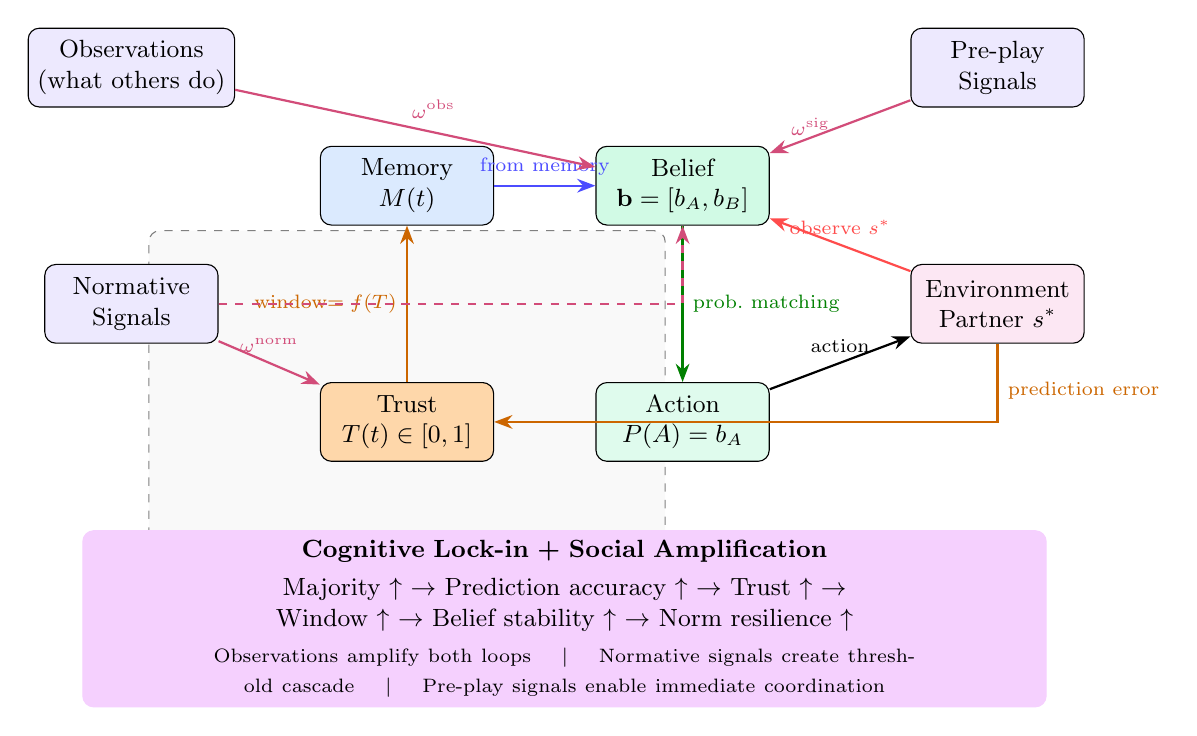
\begin{tikzpicture}[
    >=Stealth,
    box/.style={draw, rounded corners, minimum width=2.2cm, minimum height=1cm, align=center, font=\small},
    arrow/.style={->, thick},
    label/.style={font=\scriptsize, midway},
    every node/.style={font=\small}
]

% ---- Agent Internal State ----
\node[box, fill=memblue] (memory) at (0, 3) {Memory\\$M(t)$};
\node[box, fill=beliefgreen] (belief) at (3.5, 3) {Belief\\$\mathbf{b} = [b_A, b_B]$};
\node[box, fill=trustorange] (trust) at (0, 0) {Trust\\$T(t) \in [0,1]$};
\node[box, fill=beliefgreen!70] (action) at (3.5, 0) {Action\\$P(A) = b_A$};

% ---- Communication Layer ----
\node[box, fill=commpurple] (obs) at (-3.5, 4.5) {Observations\\(what others do)};
\node[box, fill=commpurple] (norm) at (-3.5, 1.5) {Normative\\Signals};
\node[box, fill=commpurple] (signal) at (7.5, 4.5) {Pre-play\\Signals};

% ---- Environment ----
\node[box, fill=envpink] (env) at (7.5, 1.5) {Environment\\Partner $s^*$};

% ---- Agent boundary ----
\begin{scope}[on background layer]
    \node[draw=gray, dashed, rounded corners, fill=gray!5,
          fit=(memory)(belief)(trust)(action),
          inner sep=12pt, label={[font=\small\bfseries]above:AGENT}] {};
\end{scope}

% ---- Internal arrows ----
\draw[arrow, blue!70] (memory) -- node[label, above] {from memory} (belief);
\draw[arrow, green!50!black] (belief) -- node[label, right] {prob.\ matching} (action);
\draw[arrow, orange!80!black] (trust) -- node[label, left] {window\\$= f(T)$} (memory);

% ---- Environment arrows ----
\draw[arrow, red!70] (env) -- node[label, above] {observe $s^*$} (belief);
\draw[arrow] (action) -- node[label, above] {action} (env);
\draw[arrow, orange!80!black] (env) |- node[label, near start, right, yshift=-3pt] {prediction error} (trust);

% ---- Communication arrows ----
\draw[arrow, purple!70] (obs) -- node[label, above right, xshift=-5pt] {$\omega^{\text{obs}}$} (belief);
\draw[arrow, purple!70] (norm) -- node[label, above] {$\omega^{\text{norm}}$} (trust);
\draw[arrow, purple!70, dashed] (norm) -| node[label, near start, above] {} (belief);
\draw[arrow, purple!70] (signal) -- node[label, left] {$\omega^{\text{sig}}$} (belief);

% ---- Lock-in annotation ----
\node[draw=lockinpink, fill=lockinpink, rounded corners, text width=12cm, align=center, font=\small] at (2, -2.5) {
    \textbf{Cognitive Lock-in + Social Amplification}\\[3pt]
    Majority $\uparrow$ $\to$ Prediction accuracy $\uparrow$ $\to$ Trust $\uparrow$ $\to$ Window $\uparrow$ $\to$ Belief stability $\uparrow$ $\to$ Norm resilience $\uparrow$\\[2pt]
    {\scriptsize Observations amplify both loops \quad $|$ \quad Normative signals create threshold cascade \quad $|$ \quad Pre-play signals enable immediate coordination}
};

\end{tikzpicture}
\caption{Unified model architecture. Trust is the central state variable controlling memory window (cognitive lock-in). Communication channels feed into belief formation and modulate trust dynamics (social amplification). Action selection uses probability matching---behaviorally neutral, enabling clean attribution.}
\label{fig:unified}
\end{figure}

% =====================================================================
\section{Summary}
% =====================================================================

\subsection*{The Model in One Paragraph}

Agents in a coordination game form beliefs from memory of past interactions. Trust, updated by prediction accuracy with asymmetric dynamics ($\alpha < \beta$), controls how much history the agent considers (memory window). This creates \textbf{cognitive lock-in}: successful coordination raises trust, expands memory, stabilizes beliefs, and makes the norm resistant to reversal. Communication adds \textbf{social amplification}: observations let agents learn from the population (weighted by inverse trust, per \citeauthor{rendell2010copy}'s ``copy when uncertain''); normative signals create shared expectations about what one \emph{should} do (enabling true norms per \citeauthor{bicchieri2006grammar}); pre-play signals coordinate immediate interaction. Communication modulates trust dynamics rather than entering memory, consistent with \citeauthor{behrens2008social}'s finding that social and reward prediction errors share a common learning-rate modulator. The result is a model where cognitive lock-in explains norm \emph{stability}, social amplification explains norm \emph{speed}, and their combination produces self-enforcing social norms from cold start.

\subsection*{Key Equations}

\begin{align*}
\text{Action:} && P(s_i = A) &= b_A && \text{(probability matching)} \\
\text{Trust:} && T^* &= \frac{p\alpha}{p\alpha + (1-p)\beta} && \text{(steady state)} \\
\text{Window:} && w &= \text{base} + \lfloor T \times (\text{max} - \text{base}) \rfloor && \text{(cognitive lock-in)} \\
\text{Belief:} && \mathbf{b} &= (1-\omega^{\text{norm}}) \cdot \mathbf{b}^{\text{emp}} + \omega^{\text{norm}} \cdot \mathbf{b}^{\text{norm}} && \text{(integration)} \\
\text{Trust update:} && \Delta T &= \delta^{\text{base}} \cdot (1 + \gamma_{\text{obs}} \cdot a) - \delta \cdot \mathbf{1}[\text{deviate}] \cdot c^2 && \text{(full)}
\end{align*}

% =====================================================================
\bibliographystyle{apalike}
\begin{thebibliography}{99}

\bibitem[Behrens et al.(2007)]{behrens2007learning}
Behrens, T.~E.~J., Woolrich, M.~W., Walton, M.~E., \& Rushworth, M.~F.~S. (2007).
Learning the value of information in an uncertain world.
\textit{Nature Neuroscience}, 10(9), 1214--1221.

\bibitem[Behrens et al.(2008)]{behrens2008social}
Behrens, T.~E.~J., Hunt, L.~T., Woolrich, M.~W., \& Rushworth, M.~F.~S. (2008).
Associative learning of social value.
\textit{Nature}, 456(7219), 245--249.

\bibitem[Bicchieri(2006)]{bicchieri2006grammar}
Bicchieri, C. (2006).
\textit{The Grammar of Society: The Nature and Dynamics of Social Norms}.
Cambridge University Press.

\bibitem[Camerer \& Ho(1999)]{camerer1999ewa}
Camerer, C.~F., \& Ho, T.~H. (1999).
Experience-weighted attraction learning in normal form games.
\textit{Econometrica}, 67(4), 827--874.

\bibitem[Centola et al.(2018)]{centola2018tipping}
Centola, D., Becker, J., Brackbill, D., \& Baronchelli, A. (2018).
Experimental evidence for tipping points in social convention.
\textit{Science}, 360(6393), 1116--1119.

\bibitem[Henrich \& Boyd(1998)]{henrich1998conformist}
Henrich, J., \& Boyd, R. (1998).
The evolution of conformist transmission and the emergence of between-group differences.
\textit{Evolution and Human Behavior}, 19(4), 215--241.

\bibitem[Miller(1956)]{miller1956magical}
Miller, G.~A. (1956).
The magical number seven, plus or minus two.
\textit{Psychological Review}, 63(2), 81--97.

\bibitem[Rendell et al.(2010)]{rendell2010copy}
Rendell, L., Boyd, R., Cownden, D., et al. (2010).
Why copy others? Insights from the social learning strategies tournament.
\textit{Science}, 328(5975), 208--213.

\bibitem[Skyrms(2010)]{skyrms2010signals}
Skyrms, B. (2010).
\textit{Signals: Evolution, Learning, and Information}.
Oxford University Press.

\bibitem[Slovic(1993)]{slovic1993perceived}
Slovic, P. (1993).
Perceived risk, trust, and democracy.
\textit{Risk Analysis}, 13(6), 675--682.

\bibitem[Toelch \& Dolan(2015)]{toelch2015informational}
Toelch, U., \& Dolan, R.~J. (2015).
Informational and normative influences in conformity from a neurocomputational perspective.
\textit{Trends in Cognitive Sciences}, 19(10), 579--589.

\bibitem[Toyokawa et al.(2019)]{toyokawa2019conformist}
Toyokawa, W., Whalen, A., \& Laland, K.~N. (2019).
Social learning strategies regulate the wisdom and madness of interactive crowds.
\textit{Nature Human Behaviour}, 3(2), 183--193.

\bibitem[Young(1993)]{young1993evolution}
Young, H.~P. (1993).
The evolution of conventions.
\textit{Econometrica}, 61(1), 57--84.

\end{thebibliography}

\end{document}
